\documentclass[a4paper]{myarticle}

\title{%
  CS7.301: Assignment 2 \\
  \Large Bias-Variance Tradeoff}
\author{Himanshu Singh (2023121013)}
\date{\today}

\begin{document}

\maketitle

\section{Gradient Descent}

Gradient descent is an iterative algorithm used in optimization, specifically to minimize the so called ``cost function''. In the case of linear regression, we typically seek to minimize the mean square error, given by the following function:

\begin{align*}
L & = \dfrac{1}{n}\sum_{i=1}^{n} (\hat{f}(x_i) - y_i)^2 \\
& = \dfrac{1}{n}\sum_{i=1}^{n} (\textbf{w}^T\textbf{x} - y_i)^2
\end{align*}

We assume the input vector is a $d+1$ dimensional vector, starting with a constant 1, to accomodate for the bias term $w_0$. We start with an initial estimate for the optimization variables ${w_i}$ and update them according to the following equation:

$$w_i = w_i - \alpha\dfrac{\partial L}{\partial w_i}$$

Here, $\alpha$ is called the step size, and the partial derivatives give us the descent direction. This can equivalently be written in vector notation, i.e. in terms of the gradient vector.

$$\textbf{w} = \textbf{w} - \alpha\nabla_w L$$

We apply this iteratively until a stopping condition is satisfied, say we have achieved the minima, i.e. $\nabla_w L = 0$, or more practically  $\norm{\nabla_w L} \leq \epsilon$, for some $\epsilon > 0$.

The analytical solution for linear regression, obtained by solving $\nabla_w L = 0$, is given by:

$$\textbf{w} = (\textbf{X}^T\textbf{X})^{-1} \textbf{X}^T\textbf{y}$$

Here, $\textbf{X}$ and $\textbf{y}$ represent the vector of (the possibly multivariate) training input and output points respectively.

\section{Numerical on Bias and Variance}

\begin{table}[H]
\centering
\renewcommand{\arraystretch}{1.5}
\begin{tabularx}{\linewidth}{LLLLLccc}
\hline
$x$ & $y$ & $f_1(x)$ & $f_2(x)$ & $f_3(x)$ & $\E_i[f_i(x)]$ & $\E_i[f_i(x)] - y$ & $[\E_i[f_i(x)] - y]^2$ \\
\hline
-2 & 5 & 3 & -2 & 5 & 2 & -3 & 9 \\
-1 & 0 & 0 & -2 & 1 & -0.33 & -0.33 & 0.11 \\
0 & 1 & 1 & 0 & 1 & 0.66 & -0.33 & 0.11 \\
1 & 4 & 6 & 4 & 5 & 5 & 1 & 1 \\
2 & 11 & 15 & 10 & 13 & 12.66 & 1.66 & 2.77 \\
3 & 22 & 28 & 18 & 25 & 23.66 & 1.66 & 2.77 \\
\hline
& & & & & & & 2.63 \\
\hline
\end{tabularx}
\caption{Calculation of Bias\textsuperscript{2}}
\label{tab:q2a}
\end{table}

\begin{table}[H]
\centering
\renewcommand{\arraystretch}{1.5}
\begin{tabularx}{\linewidth}{Lcccc}
\hline
$x$ & $(f_1(x) - \E_i[f_i(x)])^2$ & $(f_2(x) - \E_i[f_i(x)])^2$ & $(f_3(x) - \E_i[f_i(x)])^2$ & $\E_i[(f_i(x) - \E_i[f_i(x)])^2]$ \\
\hline
-2 & 1 & 16 & 9 & 8.66 \\
-1 & 0.11 & 2.77 & 1.77 & 1.55 \\
0 & 0.11 & 0.44 & 0.11 & 0.22 \\
1 & 1 & 1 & 0 & 0.66 \\
2 & 5.44 & 7.11 & 0.11 & 4.22 \\
3 & 18.77 & 32.11 & 1.77 & 17.55 \\
\hline
& & & & 5.48 \\
\hline
\end{tabularx}
\caption{Calculation of Variance}
\label{tab:q2b}
\end{table}

\begin{table}[H]
\centering
\renewcommand{\arraystretch}{1.5}
\begin{tabularx}{\linewidth}{cLLLL}
\hline
$x$ & $(y - f_1(x))^2$ & $(y - f_2(x))^2$ & $(y - f_3(x))^2$ & $\E_i[(y - f_i(x))^2]$ \\
\hline
-2 & 4 & 49 & 0 & 17.66 \\
-1 & 0 & 4 & 1 & 1.66 \\
0 & 0 & 1 & 0 & 0.33 \\
1 & 4 & 0 & 1 & 1.66 \\
2 & 16 & 1 & 4 & 7 \\
3 & 36 & 16 & 9 & 20.33 \\
\hline
& & & & 8.11 \\
\hline
\end{tabularx}
\caption{Calculation of MSE}
\label{tab:q2c}
\end{table}

See \autoref{tab:q2a}, \autoref{tab:q2b} and \autoref{tab:q2c}. Thus, we conclude that MSE = Bias\textsuperscript{2} + Variance, for the given data.

\section{Calculating Bias and Variance}
\label{sec:q3}

We can observe that bias decreases rapidly, as we bring the degree of polynomial down to 3. This is also accompanied with a decrease in MSE (see \autoref{tab:q4}). This points to a strong possibility that the test data can most accurately be modeled using a polynomial of degree 3.

Variance, as one would expect, increases with increase in model complexity. This results in a regular increase in MSE (see \autoref{tab:q4}), after degree = 3, when the sharp decrease in Bias\textsuperscript{2} had stagnated. Notably, bias increases rapidly, after degree = 8, possibly as the model tries to overfit on the noise.

\begin{table}[H]
\centering
\renewcommand{\arraystretch}{1.5}
\begin{tabularx}{\linewidth}{Lccc}
\hline
Degree of Polynomial & Average Bias & Average Bias\textsuperscript{2} & Average Variance \\
\hline
1 & -0.23648566043247068 & 0.9936640602861002 & 0.07953765467730094 \\
2 & -0.23065115241058906 & 0.9481028389983889 & 0.10697227621961831 \\
3 & 0.022023412996105995 & 0.017391283982556432 & 0.11912286770019158 \\
4 & -0.008031184511968848 & 0.027668586044199573 & 0.19250257249294855 \\
5 & -0.01009935641279951 & 0.028914548854186456 & 0.20951057588851082 \\
6 & -0.005727057309104389 & 0.02906706046367728 & 0.25042806449044935 \\
7 & -0.009345566968466335 & 0.031021600796763794 & 0.30112437488602656 \\
8 & -0.02610912867775783 & 0.04824938814996045 & 0.24500478677746512 \\
9 & -0.057305823747988094 & 0.12234505440502912 & 0.24395941553756498 \\
10 & -0.08794196460108164 & 0.2908053168874439 & 0.2539041076577705 \\
\hline
\end{tabularx}
\caption{Average Bias and Variance of models, versus their Degree of Polynomial}
\label{tab:q3}
\end{table}

\section{Calculating Irreducible Error}
\label{sec:q4}

Irreducible error is associated with the inherent randomness/noise/variability in the data that cannot be explained by the features or predictors in the model. The minor fluctuations in the irreducible error, tabulated here, with change in model, are indeed a manifestation of this randomness.

\begin{table}[H]
\centering
\renewcommand{\arraystretch}{1.5}
\begin{tabularx}{\linewidth}{cLL}
\hline
Degree of Polynomial & Average MSE & Average Irreducible Error \\
\hline
1 & 1.0732017149634019 & 7.355227538141662e-16 \\
2 & 1.0550751152180062 & -9.575673587391975e-16 \\
3 & 0.13651415168274794 & -6.938893903907228e-17 \\
4 & 0.22017115853714825 & 1.1102230246251565e-16 \\
5 & 0.23842512474269725 & -2.7755575615628914e-17 \\
6 & 0.2794951249541265 & -1.6653345369377348e-16 \\
7 & 0.33214597568279014 & -2.220446049250313e-16 \\
8 & 0.29325417492742545 & -1.1102230246251565e-16 \\
9 & 0.36630446994259414 & 2.7755575615628914e-17 \\
10 & 0.5447094245452146 & 2.7755575615628914e-16 \\
\hline
\end{tabularx}
\caption{MSE and Irreducible Error of models, versus their Degree of Polynomial}
\label{tab:q4}
\end{table}

\section{Plotting Bias\textsuperscript{2} - Variance Graph}

Similar observations from \autoref{sec:q3} follow. The underlying test data seems to be more aligned with polynomial of degree 3. The high bias for degree \textless{} 3 indicate underfitting of data. On the other hand, the high variance and still increasing bias, for degree \textgreater{} 8 indicate overfitting, with the model not generalizing on the larger patterns, and trying to fit on the noise present in the training data. The reasonably good bias and variance for degree $\in [3, 8]$ suggest that models with higher degree polynomials are choosing to simulate the effect of a cubic function, to a great extent, rather than exploring drastically different combinations.

\begin{figure}[H]
  \centering
  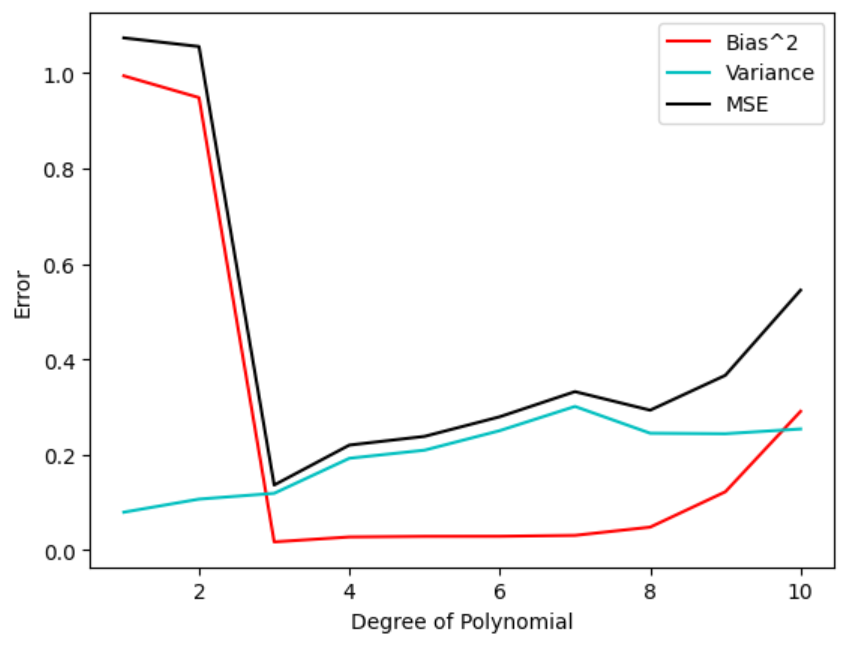
\includegraphics[width=0.65\textwidth]{plot.png}
  \caption{Plot variation of Bias\textsuperscript{2}, Variance and MSE, versus Degree of Polynomial}
  \label{fig:q5}
\end{figure}

\end{document}
